\documentclass[12pt]{article}


\usepackage{graphics}
\usepackage{graphicx}

\begin{document}

\title{Hazards in Combinational Logic}
\maketitle

If the input of a combinational circuit changes, unwanted switching variations may appear in the output. These variations occur when different paths from the input to output have different delays. If, from response to a single input change and for some combination of propagation delay, an output momentarily goes to 0 when it should remain a constant value of 1, the circuit is said to have a static 1-hazard. Likewise, if the output momentarily goes to 1 when it should remain at a constant value of 0, the circuit is said to have a 0-hazard.

When an output is supposed to change values from 0 to 1, or 1 to 0, this output may change three or more times; if this situation were to occur, the circuit is said to have a dynamic hazard. Figure 1.1 shows the different outputs from a circuit with hazards. In each of the three cases, the steady-state output of the circuit is correct, however, a switching variation appears at the circuit output when the input is changed. 



\begin{center}
	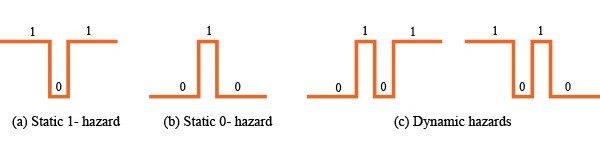
\includegraphics[scale=0.8]{./Static-and-dynamic-hazards-1.jpg}
	%\caption{Figure 1.1 }
\end{center}

The first hazard in Figure 1.2, the static 1-hazard depicts that if A = C = 1, then F = B + B'  = 1, thus the output F should remain at a constant 1 when B changed from 1 to 0. However in the next illustration, the static 0-hazard , if each gate has a propagation of 10 ns, E will go to 0 before D goes to 1, resulting in a momentary 0 appearing at output F. This is also known to be a glitch caused by the 1-hazard. One should note that right after B changes to 0, both the inverter input (B) and output (B') are 0 until the delay has elapsed. During this propagation period, both of these input terms in the equation for F have value of 0, so F also momentarily goes to a value of 0.

These hazards, static and dynamic, are completely independent of the propagation delays that exist in the circuit. If a combinational circuit has no hazards, then it is said that for any combination of propagation delays and for any individual input change, that output will not have a variation in I/O value. On the contrary, if a circuit were to contain a hazard, then there will be some combination of delays as well as an input change for which the output in the circuit contains a transient.

This combination of delays that produce a glitch may or may not be likely to occur in the implementation of the circuit. In some instances it is very unlikely that such delays would occur. The transients (or glitches) that result from static and dynamic timing hazards very seldom cause problems in fully synchronous circuits, but they are a major issue in asynchronous circuits (which includes nominally synchronous circuits that involve either the use of asynchronous preset/reset inputs that use gated clocks).

The variation in input and output also depends on how each gate will respond to a change of input value. In some instances, if more than one input gate changes within a short amount of time, the gate may or may not respond to the individual input changes. One example in Figure 1.2, assuming that the inverter (B) has a propagation delay of 2ns instead of 10ns. Then input D and E changes reaching the output OR gate are 2ns from each other, thus the OR gate may or may not generate the 0 glitch. 



\begin{center}
	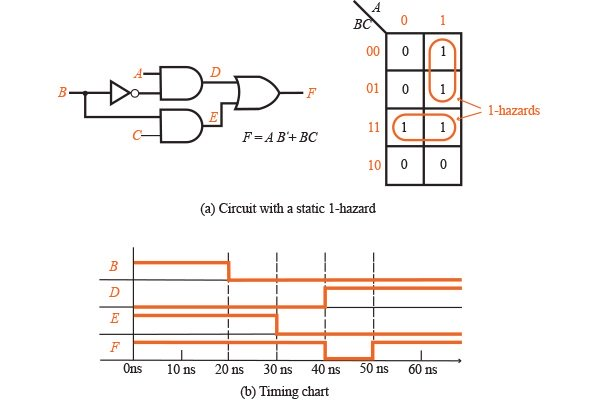
\includegraphics[scale=0.8]{./static-hazard-timing-chart.jpg}
	%\caption{Figure 1.2 }
\end{center}


A gate displaying this type of response is said to have what is known as an inertial delay. Rather often the inertial delay value is presumed to be the same as the propagation delay of the gate. When this occurs, the circuit above will respond with a 0 glitch only for inverter propagation delays that are larger than 10ns. However, if an input gate invariably responds to input change that has a propagation delay, is said to have an ideal or transport delay. If the OR gate shown above has this type of delay, than a 0 glitch would be generated for any nonzero value for the inverter propagation delay.

Hazards can always be discovered using a Karnaugh map. The map illustrated above in Figure 1.2, which not a single loop covers both minterms ABC and AB'C. Thus if A = C = 1 and B's value changes, both of these terms can go to 0 momentarily; from this momentary change, a 0 glitch is found in F. To detect hazards in a two-level AND-OR combinational circuit, the following procedure is completed: 

A sum-of-products expression for the circuit needs to be written out.
Each term should be plotted on the map and looped, if possible.
If any two adjacent 1's are not covered by the same loop, then a 1-hazard exists for the transition between those two 1's. For any n variable map, this transition only occurs when one variable changes value and the other n  1 variables are held constant. 

If another loop is added to the Karnaugh map in Fig. 1.2(a) and then add the corresponding gate to the circuit in Figure 1.3 below, the hazard can be eliminated. The term AC remains at a constant value of 1 while B is changing, thus a glitch cannot appear in the output. With this change, F is no longer a minimum SOP. 



\begin{center}
	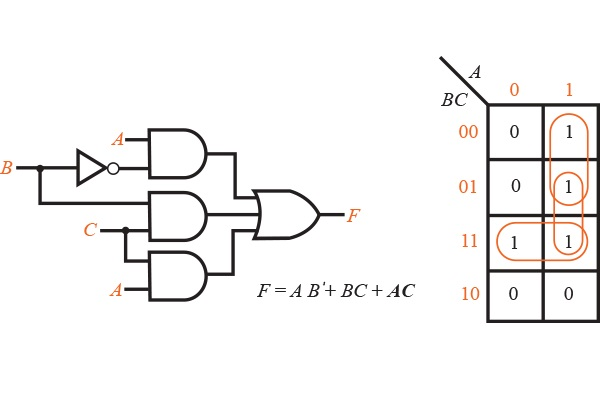
\includegraphics[scale=0.8]{./karnaugh-map-1-3.jpg}
	%\caption{Figure 1.3 }
\end{center}


Figure 1.4(a) is a circuit with numerous 0-hazards. The function that represents the circuit's output is:

F  = (A + C)(A' + D')(B' + C' + D)


The Karnaugh map in Fig. 1.4(b) has four pairs of adjacent 0's that are not covered by a common loop. The arrows indicate where each 0 is not being looped, and they each correspond to a 0-hazard. If A = 0, B = 1, D = 0, and C changes from 0 to 1, there is a chance that a spike can appear at the output for any combination of gate delays. lastly, Fig. 1.4(c) depicts a timing diagram that, assumes a delay of 3ns for each individual inverter and a delay of 5ns for each AND gate and each OR gate.



\begin{center}
	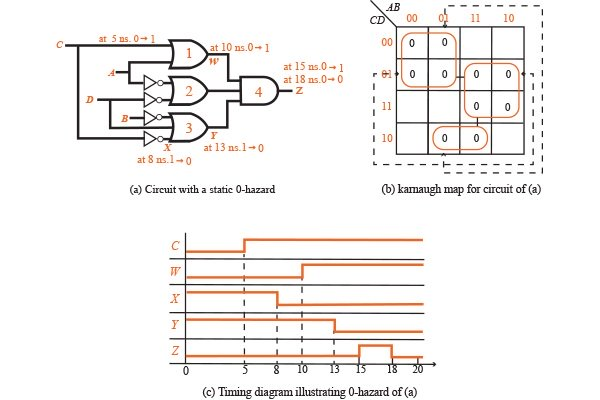
\includegraphics[scale=0.8]{./Figure-1-4-static-hazard-diagrams.jpg}
	%\caption{Figure 1.4 }
\end{center}


The 0-hazards can be eliminated by looping extra prime implicants that cover the 0's adjacent to one another, as long as they are not already covered by a common loop. By eliminating algebraically redundant terms, or consensus terms, the circuit can be reduced to the following equation below. Using three additional loops will completely eliminate the 0-hazards, resulting the following equation: 


F = (A + C)(A' + D')(B' + C' + D)(C + D')(A + B' + D)(A' + B' + C')


This figure below illustrates the Karnaugh map after removing the 0-hazards. 



\begin{center}
	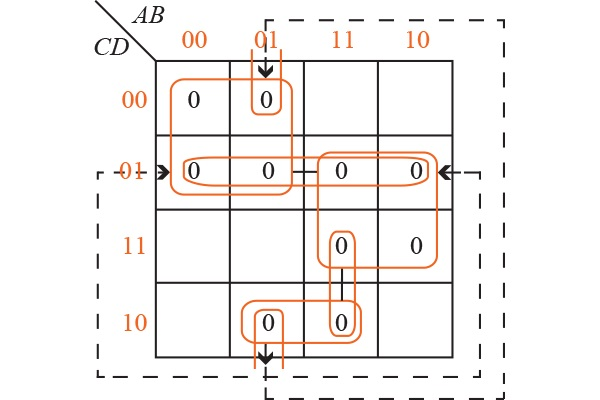
\includegraphics[scale=0.8]{./karnaugh-map-1-5.jpg}
	%\caption{Figure 1.5 }
\end{center}


\section{Testing of Logic Circuits}

An essential component of designing logic circuits is making sure that the final design is correct and correcting if necessary. To test a circuit, one can either build them or simulate them on a digital computer. Computer simulation is generally faster and more economical because you do not have to waste money on components. As the complexity of the circuit increases, it becomes very important to simulate a design before actually building it. When a design is built in integrated circuit form, it is essential to simulate because fabricating an integrated circuit can take a very long time and correcting errors can be an expensive fix. Simulation is done before the actual build for many reasons: confirmation that the design is correct logically, making sure that the timing of all logic signals are correct, and verification of faulty components in the circuit as an aid to finding tests for the circuit. 

In order to simulate a logic circuit design, there are specific programs needed in order to build the design on the computer. First, any components and connects to the logic inputs and outputs need to be specified. After that, these inputs can then be specified. Lastly, the circuit outputs should be reviewed to correct any mistakes. A specific description of the circuit may be inputted into the computer simulation program as to the list of any connections between logic elements, or it may be in the form of a drawn logic diagram on the computer screen. 

A simple computer simulation program for a set of combinational logic may look like this:

The inputs of the circuit are implemented to the first set of gates in the circuit, and the output values of those gates are then calculated.
These outputs which changed in the first step are then fed into the next level (or set) of gate inputs. If any input has changed, then that same input's value is calculated.
The previous step is repeated until there isn't a single change in gate input values. When this is met, the circuit is said to be in steady-state condition, and finally the output values may be read.
Steps 1-3 are repeated every time there is a change in an input. 





\end{document}